\chapter{Performance}
\label{chap:perfux}
The content of this chapter shows performance measurements made by author regarding Test Sheets processing (generation of executable javascript file from the spreadsheet file) and tests execution.  
All measurements were made on hardware with following characteristics:
\begin{itemize}
	\item Mac mini (Late 2014)
	\item \textbf{Processor:} 2.6 GHz Intel Core i5;
	\item \textbf{Memory:} 8 GB 1600 MHz DD3;
	\item \textbf{Storage:}  1 TB SATA Disk.
\end{itemize}

The characteristics of the tests' execution environment are following:
\begin{itemize}
\item Operational System:
\begin{itemize}
	\item OS X El Capitan
	\item version 10.11.4
\end{itemize}

\item node.js environment:
\begin{itemize}
	\item node version 4.4.5
	\item npm version 2.15.5
\end{itemize}
\end{itemize}


\section{Generation performance}
In this section we describe the system's performance characteristics for generating executable javascript files from the Test Sheet xlsx files. The performance was measured for two cases: the first case is when all the Test Sheet files are located in a single (root) directory, the second case when root directory contains Test Sheet files and another folder with Test Sheet files and yet another folder.
\paragraph{Single folder} - all files are located within the same (root) directory (Diagram: \ref{fig:gs}).
\begin{itemize}
	\item \textbf{New} - all the files are newly added on the every iteration of the measurement with deletion of all the previously generated javascript files. Thus the number of generated js files is equivalent to the number of files in a directory.
	\item \textbf{Add} - only ten xlsx files are added on every iteration of the measurement processes. Thus previously added xlsx files are skipped for javascript files creation. All generated files are skipped as files with non xlsx extension.
\end{itemize}


\begin{figure}[ht]
	\label{fig:gs}
	\centering
	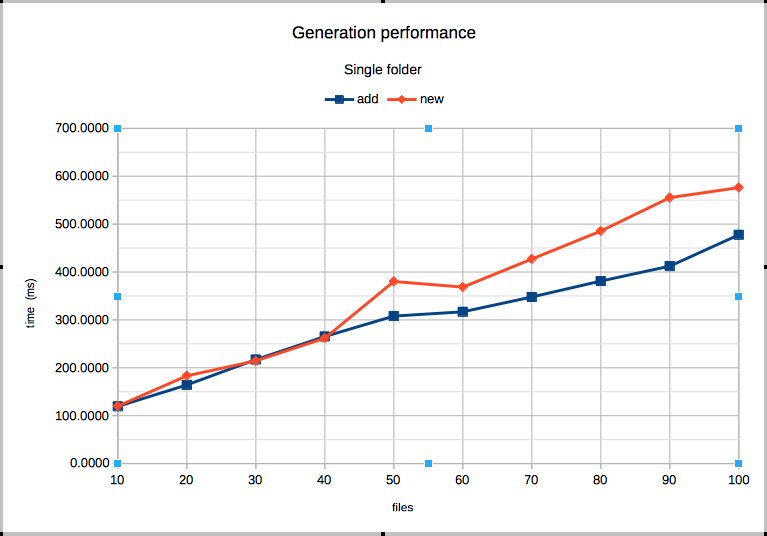
\includegraphics[width=\textwidth]{grafiken/generation_single}
	\caption{Generation performance for files within single folder}
\end{figure}

\paragraph{Nested folder} - each folder contains ten xlsx files and another folder with the same content (Diagram: \ref{fig:gn}).
\begin{itemize}
	\item \textbf{New} - all the files are newly added on the every iteration of the measurement with deletion of previously generated javascript files. Thus the number of created javascript files is equivalent to the number of files in a directory and nested folder(s).
	\item \textbf{Add} - ten xlsx files with the folder nested within the folder created inside the directory from the previous iteration are added. Thus previously added xlsx files are skipped for  the javascript files creation. The javascript files are generated only for the folder with the deepest level of nesting.
\end{itemize}


\begin{figure}[ht]
	\label{fig:gn}
	\centering
	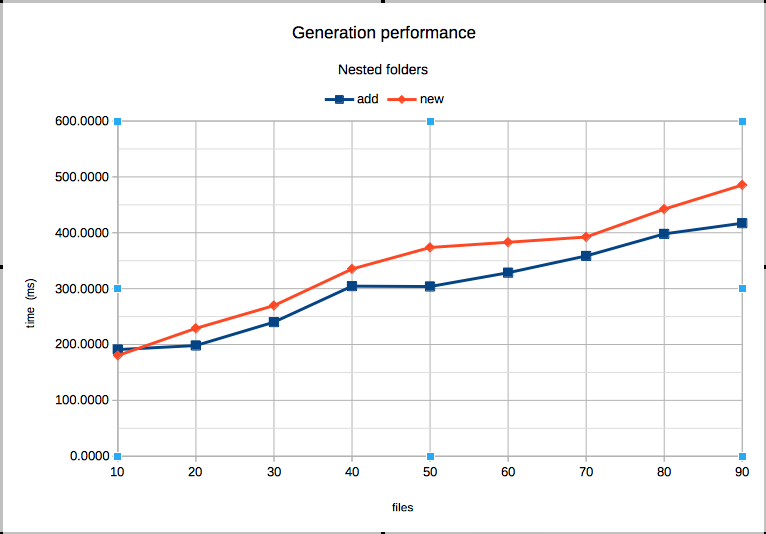
\includegraphics[width=\textwidth]{grafiken/generation_nested}
	\caption{Generation performance for files within nested folders}
\end{figure}

\section{Executions performance}
This section shows execution performance measured for the javascript files generated from the Test Sheet file. All the files are located within the same folder. The measurements were done for two extreme cases of test steps definitions. The first case, when all test step are independent from each other thus can be invoked for execution within the same iteration of the event loop. The second case, when input of all test steps except the first is defined by the result of the previous test step. Thus, there is only one test step called per event loop iteration and the amount of iterations is equal to the number of test steps.
All measurements are done for both deep and scheme only comparisons.

\paragraph{Independent test steps} - all test steps are independent from each other. For this reason their calls are done within the same iteration of an event loop (Diagram: \ref{fig:ei}).
\begin{itemize}
	\item \textbf{Scheme comparison} - actual and expected outputs are compared by their scheme
	\item \textbf{Deep comparison} - actual and expected outputs are compared by their scheme and values of every property
\end{itemize}
\begin{figure}[ht]
	\label{fig:ei}
	\centering
	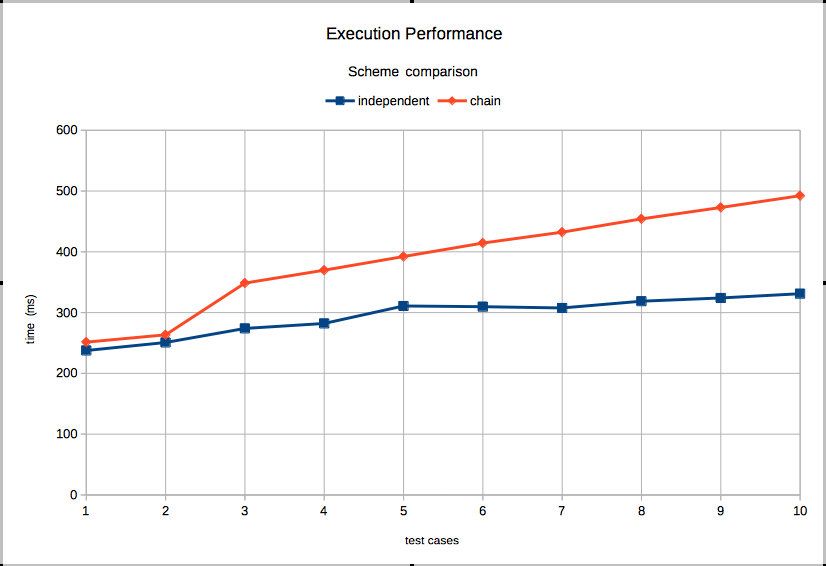
\includegraphics[width=\textwidth]{grafiken/exec_scheme}
	\caption{Execution performance for independent test steps}
\end{figure}

\paragraph{Chain relationship} - output of each test step (except the first) defines input for row below. Therefore there is one execution call per each iteration of the event loop (Diagram: \ref{fig:ef}).
\begin{itemize}
	\item \textbf{Scheme comparison} - actual and expected outputs are compared by their scheme
	\item \textbf{Deep comparison} - actual and expected outputs are compared by their scheme and values of every property
\end{itemize}

\begin{figure}[ht]
	\label{fig:ef}
	\centering
	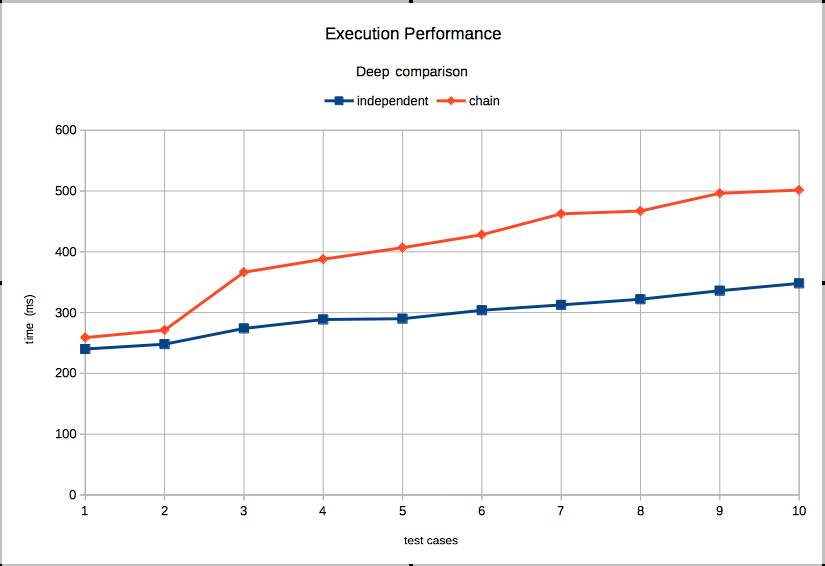
\includegraphics[width=\textwidth]{grafiken/exec_deep}
	\caption{Execution performance for interdependent test steps}
\end{figure}

The measurements from the first section shows that the Test Sheets can be structured within the root folder in arbitrary way without big looses in the generation performance. This should give positive impact on the processes of tests creation and maintenance.

The performance for tests execution proves the necessity of execution order optimization implemented within the \textit{scheme} module. It also shows that type of comparison does not influence the test execution time for small JSON object with simple structure.
